\section{Background and notation}\label{Section:Preliminaries}

The following sections aim at describing some of the required concepts and basic structures to make it easier to interpret the AMIDST models that will be presented afterwards for the different use cases. Section \ref{SubSection:HybridBNs} briefly introduces Bayesian networks and discusses the challenges encountered for reasoning with continuous and discrete variables, Section \ref{SubSection:DBNs} describes some of the basic concepts and models related to dynamic Bayesian reasoning over time, and, finally, Section \ref{SubSection:DataAnalysis} defines the data analysis techniques used to ensure a better understanding of AMIDST models.


%------------------------------------------------------------------------------------------------------------
\subsection{Graphical notation}\label{SubSection:GraphicalNotation}
%------------------------------------------------------------------------------------------------------------

Figure \ref{Figure:PreliminariesNotation} shows in the first row the graphical representation of the different types of variables used in AMIDST model classes. A continuous variable is depicted with an ellipse with a blue background, while a discrete variable is depicted with an ellipse with a green background. If a variable could be either continuous or discrete, the background of the ellipse is simultaneously blue and green. In addition, a hidden variable is depicted with a dashed-line ellipse, while an observed variable is depicted with a solid-line ellipse. Obviously, a continuous hidden variable, for example, would be represented with a blue dashed-line ellipse.

\begin{figure}[ht!]
\begin{center}
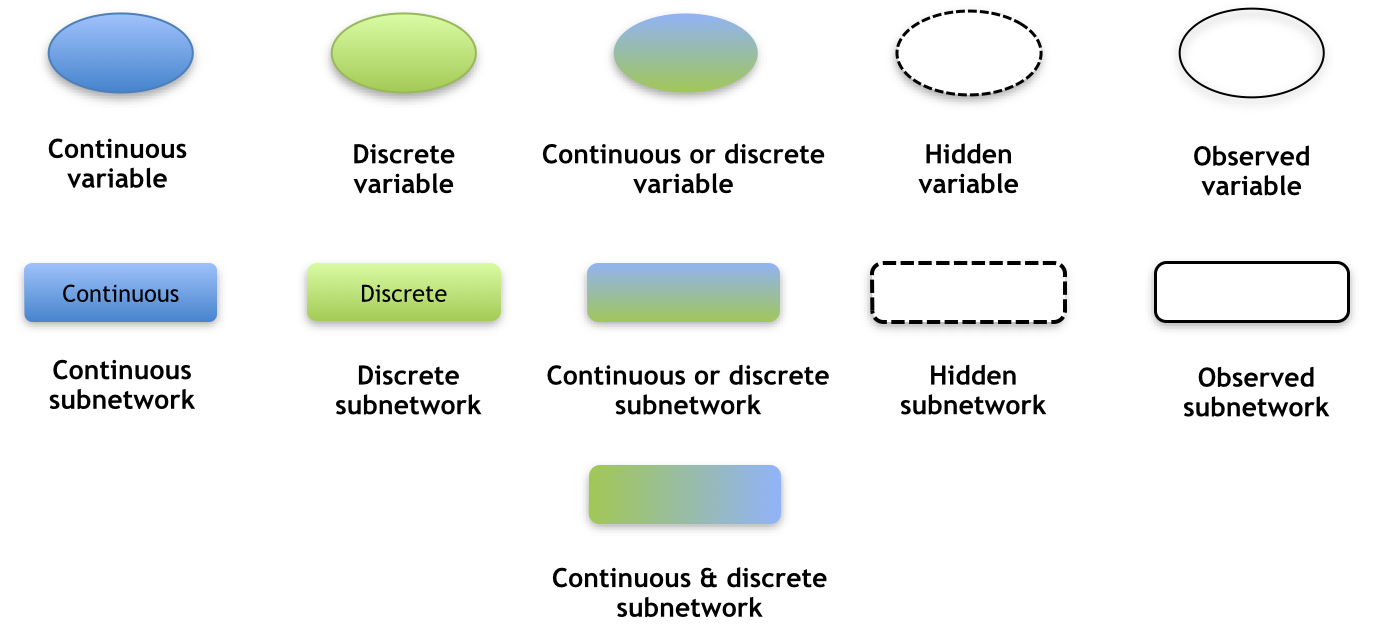
\includegraphics[scale=0.55]{./figures/PreliminariesNotation}
\caption{\label{Figure:PreliminariesNotation}Graphical notation of the different types of variables and subnetworks.
}
\end{center}
\end{figure}

The second row of Figure \ref{Figure:PreliminariesNotation} shows the graphical representation of the different types of subnetworks. A subnetwork refers to a directed acyclic graph defined over a set of variables\footnote{In particular, a subnetwork refers in our case to a part of a dynamic Bayesian network that will be defined later on this document.}. A continuous subnetwork (i.e., including only continuous variables) is depicted with a blue rectangle, while a discrete subnetwork (i.e., including only discrete variables) is depicted with a green rectangle. 

If a subnetwork can be instantiated, at a specific moment, with either continuous or discrete variables (i.e., we have a continuous or discrete subnetwork), the rectangle background is horizontally coloured with blue and green. However, if a subnetwork is simultaneously instantiated with both continuous and discrete variables (i.e., we have a continuous \& discrete subnetwork), the rectangle background is vertically coloured with blue and green. Finally, a hidden subnetwork is depicted with a dashed-line rectangle, while an observed subnetwork is depicted with a solid-line rectangle.


%------------------------------------------------------------------------------------------------------------
\subsection{Bayesian networks}\label{SubSection:HybridBNs}
%------------------------------------------------------------------------------------------------------------

Bayesian networks (BNs) \cite{JensenNielsen2007} are widely used probabilistic graphical models for reasoning under uncertainty. They graphically encode a set of conditional independence assumptions that are exploited to efficiently perform a wide variety of inference tasks such as marginal belief computation, belief updating, most probable explanation, etc.  

Formally, let $\bm X = \{X_1,\ldots,X_N\}$ denote the set of stochastic random variables defining our domain problem. A BN defines a joint distribution $P(\bm X)$ in the following form:

$$ p(\bm X) = \prod_{i=1}^N p(X_i|Pa(X_i))$$ 

\noindent where $Pa(X_i)\subset \bm X\setminus X_i$ represents the so-called \emph{parent variables} of $X_i$. Bayesian networks can be graphically represented by a directed acyclic graph (DAG). Each node, labelled $X_i$ in the graph, is associated with a factor or conditional probability $p(X_i|Pa(X_i))$. Additionally, for each parent $X_j \in Pa(X_i)$, the graph contains one directed edge pointing from $X_j$ to the \emph{child} variable $X_i$.

Figure \ref{Figure:GeneralBayesianNetwork} shows an example of a BN model. The nodes, which correspond to variables, are coloured in green or blue to highlight their nature, i.e., discrete or continuous, respectively, according to the notation depicted in Figure \ref{Figure:PreliminariesNotation}. Note that the notation on the second row corresponds to how a particular subnetwork will be represented later on in this document, e.g. a subnetwork with a set of hidden discrete and continuous variables would be represented by a dotted white frame\footnote{This is indeed the only restricted subnetwork, since only links from discrete to continuous variables are allowed and not the other way around.}. Each \textit{subnetwork module} corresponds to a part of the DBN with common features such as all the nodes are continuous and observed. Instead of eclipsed nodes used to depict single variables in a graph, we represent here the subnetwork modules using frames. In general, dashed lines refer to hidden variables or subnetworks (i.e., those including only hidden variables), while continuous lines refer to observed variables or subnetworks (i.e., those including only observed variables). Then, depending on the background colour, variables or subnetworks can be either discrete (green), continuous (blue) or hybrid (white or green/blue).

\begin{figure}[ht!]
\begin{center}
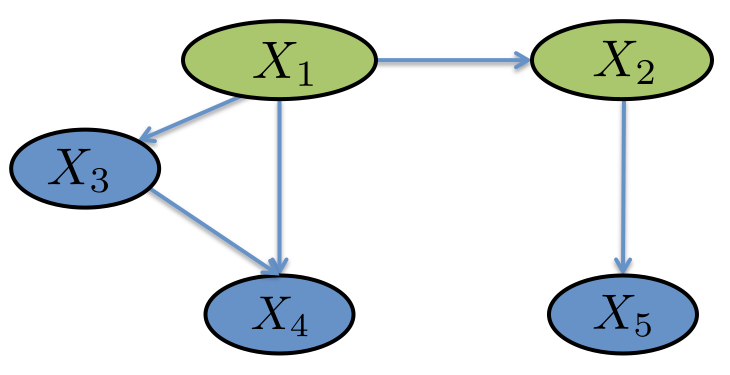
\includegraphics[scale=0.25]{./figures/PreliminariesGeneralBayesianNetwork}
\caption{\label{Figure:GeneralBayesianNetwork}Example of a BN model with continuous and discrete variables.
}
\end{center}
\end{figure}

Traditionally, BNs have been defined for discrete domains, where the entities of interest are modelled by discrete variables which ensures that belief updating can be performed efficiently and in closed form. However, this requirement imposes severe restrictions as many domains contain entities that are more appropriately modelled by variables with continuous state spaces; such as distance and velocity measurements which are key sensor readings for identifying and interpreting traffic manoeuvres (see Daimler's requirement analysis \cite{Fer14}). 

To deal with this problem, research has largely pursued three main approaches to extend BNs and support continuous variables. As a first approach, one may choose to carefully construct the model so that exact inference algorithms can still be applied. This is the case for the conditional linear Gaussian (CLG) BNs \cite{Lauritzen1992,LauritzenJensen2001}, where the local probability distributions of continuous variables are specified as conditional linear Gaussian distributions and where discrete variables can only have discrete parents. A second approach consists of considering approximate algorithms for performing inference, allowing thereby arbitrary distributions to be associated with the BN model. Examples of this approach include the Gibbs sampler \cite{Geman1984, hrycej1990gibbs} and variational inference \cite{Jordan1999}. Finally, the third approach consists of ``transforming" the original BN model into an approximate model, for which exact inference algorithms can be applied. This can be achieved either by discretizing the continuous variables \cite{KozlovKollerUAI97} or using transformations with more expressive power, such as using mixtures of truncated exponentials \cite{Moral2001} or mixtures of truncated basis functions \cite{Langseth12}.

The models presented in this deliverable, unless otherwise stated, will be parameterized according to the conditonal linear Gaussain model \cite{Lauritzen1992,LauritzenJensen2001}. That means that we will have the following conditional distributions depending of the type, continuous or discrete, of the parents and the child variables:

\begin{itemize}
\item \textbf{Discrete $\rightarrow$ Discrete}: The child variable follows an independent multinomial probability distribution for each configuration or assignment of the parents variables.

\item \textbf{Continuous $\rightarrow$ Continuous}: The child variable follows a conditional linear Gaussian distribution. I.e. the mean parameter of the Gaussian distribution of the child variable is a linear combination of the parents variables while the variance is a fixed independent parameter. 

\item \textbf{Discrete $\rightarrow$ Continuous}: In this case, the child variable is distributed as an independent Gaussian distribution for each configuration of the parents variables. 

\item \textbf{ (Discrete, Continuous) $\rightarrow$ Continuous}:  For each configuration of the discrete parents variables, the child variable follows an independent conditional Gaussian distribution depending of the continuous parents variables. I.e. the mean parameter of the Gaussian distribution of the child variable is expressed as a different linear combination of the continuous parents variables for each configuration of the discrete parents variables and, moreover, the variance of this Gaussian can also be different. 

\end{itemize}



%------------------------------------------------------------------------------------------------------------
\subsection{Probabilistic reasoning over time}\label{SubSection:DBNs}
%------------------------------------------------------------------------------------------------------------

Many domains, and in particular those being analysed in the AMIDST project, can be seen as having strong internal structure. This will be evident by the domains being appropriately described using an object oriented language, either due to repetitive substructures or substructures that can be naturally ordered in a superclass/subclass hierarchy.  Object oriented BNs \cite{KollerPfeffer1997} (OOBNs) are defined to take advantage of such internal model structure. In dynamic models, we also find this property because the same part of the model is repeated over time (i.e., we have multiple objects of the same class under the OOBNs language). A special type of OOBNs is the dynamic BN (DBN) \cite{DeanKanazawa1989}, which is used to model domains that evolve over time by representing explicitly the temporal dynamics of the system. DBNs can also be readily understood as an extension of standard BNs to the temporal domain. 

Similarly to static BNs, we model our problem/system using a set of stochastic random variables, denoted $\bm X_t$, with the main difference that variables are indexed here by a discrete time index $t$. In this way, we explicitly model the state of the system at any given time. Moreover, we always assume that the system is described at a fixed frequency, and use $\bm X_{a:b} \equiv X_a,X_{a+1},\ldots,X_{b}$ to denote the set of variables between two time points $a$ and $b$.  

For reasoning over time, we need to model the joint probability $p(\bm X_{1:T})$ which has the following natural cascade decomposition:

$$p(\bm X_{1:T})  = \prod_{t=1}^T p(\bm X_t|\bm X_{1:t-1}),$$

\noindent where $p(\bm X_t|\bm X_{1:t-1})$ is equal to $p(\bm X_1)$ for $t=1$. As $t$ increases, the conditional probability $p(\bm X_t|\bm X_{1:t-1})$ becomes intractable. Similarly to static BNs, \textit{dynamic BNs} allow more compact factorization of the above joint probability. The first kind of conditional independence assumption encoded by DBNs to reduce the factorization complexity is the well-known \textit{Markov assumption}. Under this assumption, the current state is independent from the previous one given a finite number of previous steps and the resulting models are referred to as \textit{Markov chains}. Basically, a Markov chain can be defined on either discrete or continuous variables $\bm X_{1:T}$. It exploits the following equality:

$$p(\bm X_t| \bm X_{1:t-1})  = p(\bm X_t|\bm X_{t-V:t-1})$$

\noindent where $V\geq 1$ is the order of the Markov chain. Figure \ref{Figure:markovChain} shows two examples of DBNs corresponding to first-order (i.e., $V=1$) and third-order (i.e., $V=3$) Markov chains. 

\begin{figure}[ht!]
\begin{center}
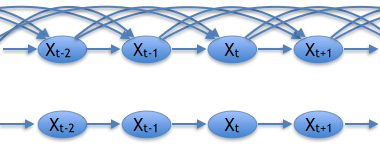
\includegraphics[scale=0.56]{./figures/PreliminariesMarkovChain}
\caption{\label{Figure:markovChain} An example of DBNs assuming a third-order (above) and a first-order (below) Markov property.
}
\end{center}
\end{figure}

Among the different kinds of Markov chains, the \textbf{first-order Markov chains} are the most widely used. They assume that knowing the present makes the future conditionally independent from the past, that is, $p(\bm X_t| \bm X_{1:t-1})  = p(\bm X_t|\bm X_{t-1})$. The problem is that this could be an unrealistic assumption in some problems leading to poor approximations of the joint distribution. One could increase the Markov order to improve the approximation at the expenses of having a more complex model. Another  alternative \cite{russelNorvig2009} would be to increase the number of variables modelling the system. This alternative is usually preferred if we have a sound understanding of the ``physics''  of the process being modelled (e.g. predicting whether it is going to rain or not tomorrow based on the raining evidence of the current day can be probably improve by considering the raining evidence of previous days. Alternatively, we can also improve this prediction by considering in the modelling the humidity and the pressure of the current day \cite{russelNorvig2009}). 

%To increase the accuracy of the approximation, one could either increase the Markov order, or equivalently, increase the number of state variables, which would consequently increase the complexity of the model in both cases. Hence, our objective is to come up with models that contain a self-sufficient set of variables, which often requires to fully understand the ``physics''  of the process being modelled for the different use cases \cite{russelNorvig2009}. 

An additional challenging problem is the specification of the conditional probabilities at each time step of the DBNs. To deal with this problem, we usually assume that changes in the world state are driven by a \textit{stationary process}, that is, $p(\bm X_{t+1}|\bm X_{t}) = p(\bm X_t|\bm X_{t-1})\ \forall t \in\{1,\ldots,T\}$. 

In the following sub-sections, we will present in more details some basic examples of DBNs, namely, \textit{hidden Markov models} (Section \ref{SubSubSection:HMMs}), \textit{Kalman filters} (Section \ref{SubSubSection:KFs}), and \textit{two-time slice DBNs} (Section \ref{SubSubSection:2DBNs}). Let us recall here that the graphical notation employed when describing all these models is depicted in Figure \ref{Figure:PreliminariesNotation}.

%-----------------------------------------------------------------------------------------------
\subsubsection{Hidden Markov models}\label{SubSubSection:HMMs}
%-----------------------------------------------------------------------------------------------

A hidden Markov model (HMM) is the simplest DBN including both hidden and observed variables, such that the latent state of the process is represented by a single discrete variable. More precisely, a HMM, shown in \ref{Figure:HMM}, defines a Markov chain over the hidden variables $X_{1:T}$. The observed variables, denoted by $\bm Y_{1:T}$, are dependent on the hidden variables under the \textit{sensor Markov assumption}, that is, $P(\bm Y_t| X_{1:T}, \bm Y_{1:T}) = P(\bm Y_t| X_t)$, where $P(\bm Y_t| X_t)$ represents the sensor (or observation) model.  

\begin{figure}[ht!]
\begin{center}
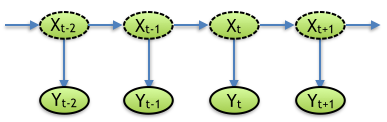
\includegraphics[scale=0.4]{./figures/PreliminariesHMM}
\caption{\label{Figure:HMM}An example of a BN structure corresponding to a HMM.}
\end{center}
\end{figure}

In that way, the joint probability distribution over the observed and hidden variables can be represented as:

\begin{equation}
P(\bm X_{1:T},\bm Y_{1:T}) = \prod_{t=1}^t{P(\bm X_t| \bm X_{t-1})P(\bm Y_t|\bm X_t)}.
\end{equation}

Although most of our models will fit into this description of observed and hidden (state) variables, there will be cases in which the transition model takes place in the observed variables (see, e.g., the case of Cajamar), which in general simplifies the learning-inference processes of the problem.

An extension of the HMM is the so-called \textit{input-output hidden Markov model} (IOHMM) shown in Figure \ref{Figure:IO-HMM}. IOHMM incorporates an extra top layer of input variables $\bm Y'_{1:T}$, which can be either continuous or discrete. The existing HMM layer of observed variables, $\bm Y_{1:T}$, is referred to as the output set of variables. 

\begin{figure}[ht!]
\begin{center}
\includegraphics[scale=0.4]{./figures/PreliminariesIO-HMM}
\caption{\label{Figure:IO-HMM}An example of a BN structure corresponding to an IO-HMM.}
\end{center}
\end{figure}

IOHMM is usually employed in supervised classification problems. In this case, both input and output variables are known during training, but only the former is known during testing. In fact, during testing, inference is performed to predict the output variables at each time step. In AMIDST we use this model in a different way. In our case, both set of input and output variables are always known, so that inference is only performed to predict the latent variables. The input variables $\bm Y'_{1:T}$ are introduced as a way to ``relax" the stationary assumption, by explicitly introducing a dependency to some observed information at each time slice, that is, the transition probability between $\bm X_t$ and $\bm X_{t+1}$ depends on the observed value $\bm Y_{t+1}$. 

%As later explained in Section \ref{Section:VerdandeModels}, we might want to further extend IOHMM model by considering a set of discrete and continuous state variables in our models. 

%-----------------------------------------------------------------------------------------------
\subsubsection{Kalman filters}\label{SubSubSection:KFs}
%-----------------------------------------------------------------------------------------------

Similar to the extension of the static BN model to hybrid domains, DBNs have likewise been extended to continuous and hybrid domains. In purely continuous domains, where the continuous variables follow linear Gaussian distributions, the DBN corresponds to (a factorized version of) a Kalman filter (KF). The structure of a KF is exactly the same as the one displayed in Figure \ref{Figure:HMM} for the HMM, however with the restriction that all variables should be continuous. In this case, the state variables can be a combination of continuous variables with different dependences, and where the dynamics of the process are assumed to be linear. 

When modelling non-linear domains, the dynamics and observational distributions are often approximated through, e.g., the \textit{extended Kalman filter}, which models the system as \textit{locally} linear in the mean of the current state distribution. Another type of model ensuring non-linear predictions with a more expressive representation is the \textit{switching Kalman filter} (SKF). The type of SKF that we are going to consider here includes an extra discrete state variable that is able to use a weighted combination of the linear sub-models. That is, the discrete state variable assigns a probability to each linear term in the mixture, hence, representing the belief state as a mixture of Gaussians. In this way, it can deal, to some extent, with violations of both the assumption of linearity and Gaussian noise. Figure \ref{Figure:SKF} depicts the graphical structure of this dynamic model.

\begin{figure}[ht!]
\begin{center}
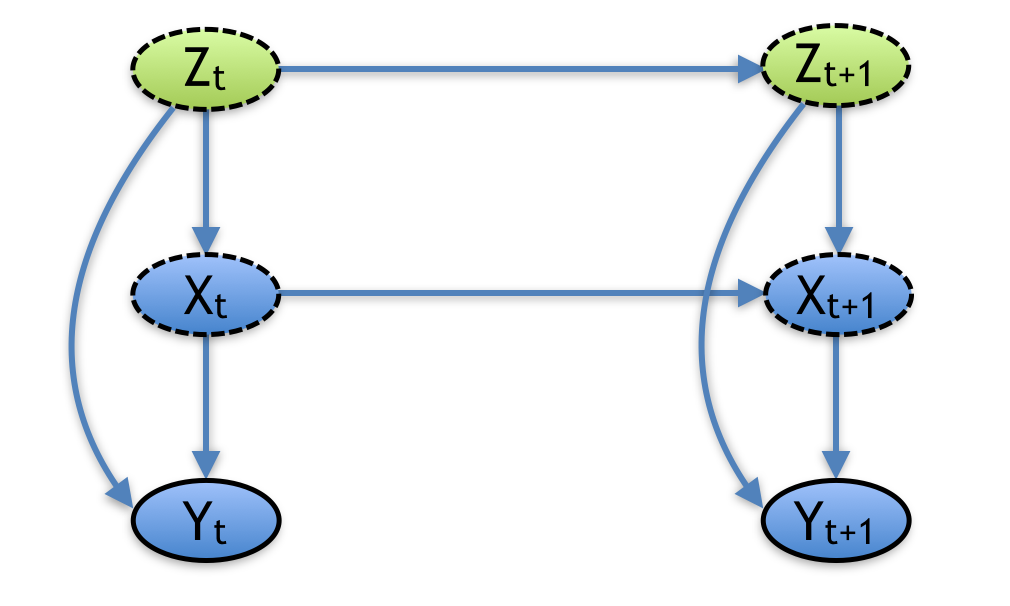
\includegraphics[scale=0.4]{./figures/PreliminariesSKF}
\caption{\label{Figure:SKF} An example of a switching Kalman filter. $Z_t$ represents the discrete state variable modelling multiple KFs running in parallel.}
\end{center}
\end{figure}

Similarly to HMM, these models can be extended by introducing an extra top layer of input variables to ``relax" the stationary assumption, by explicitly introducing a dependency to some observed information for the transition probability of the latent variables. These models will be better explained in Section \ref{Section:VerdandeModels}.

%-----------------------------------------------------------------------------------------------
\subsubsection{Two-time slice dynamic Bayesian networks}\label{SubSubSection:2DBNs}	
%-----------------------------------------------------------------------------------------------

In general, DBNs can model arbitrary distributions over time. However, in AMIDST,  we will especially focus on the so-called \textit{two-time slice DBNs} (2T-DBNs). 2T-DBNs are characterised by an \textit{initial model} representing the initial joint distribution of the process and a \textit{transition model} representing a standard BN repeated over time. This kind of DBN model satisfies both the first-order Markov assumption and the stationarity assumption. Figure \ref{Figure:DBN} shows an example of a graphical structure of a 2T-DBN model. 

\begin{figure}[ht!]
\begin{center}
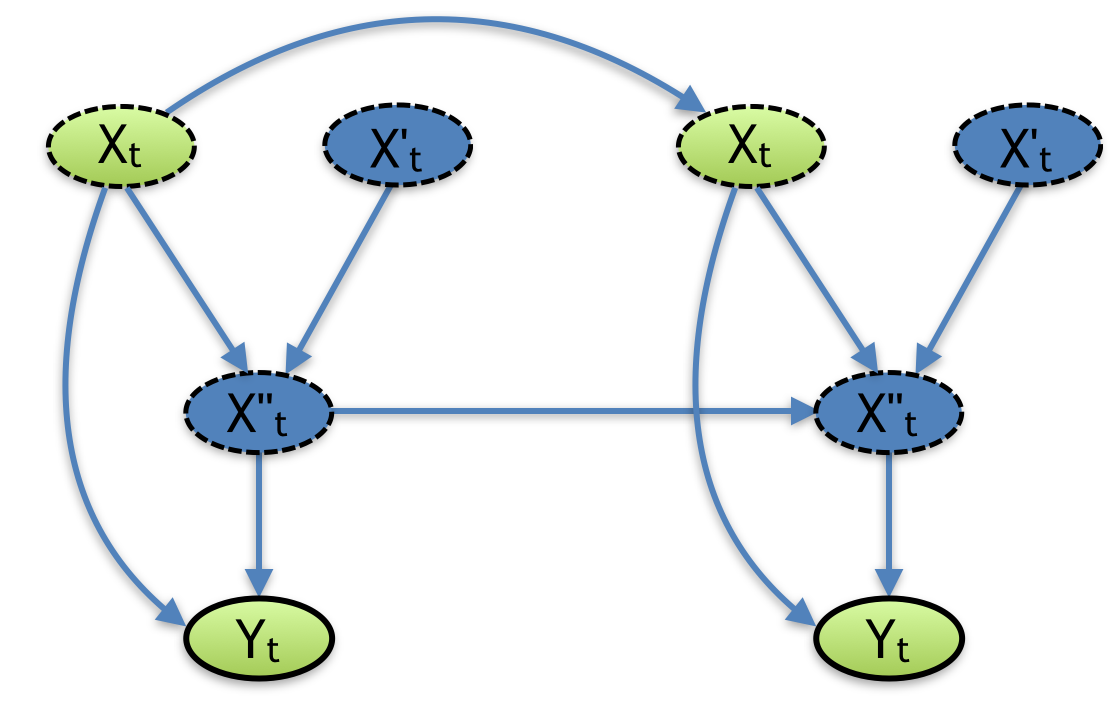
\includegraphics[scale=0.3]{./figures/PreliminariesDBN}
\caption{\label{Figure:DBN}An example of a BN structure corresponding to a 2T-DBN.}
\end{center}
\end{figure}

In a 2T-DBN, the transition distribution is represented as follows:

$$ p(\bm X_{t+1} | \bm X_t) = \prod_{X_{t+1}\in\bm X_{t+1}} p(X_{t+1}|Pa(X_{t+1})),$$ 

\noindent where $Pa(X_{t+1})$ refers to the set of parents of the variable $X_{t+1}$ in the transition model, which can be variables either at the same or the previous time step. 

Note that a HMM, KF or SKF are particular cases of a 2T-DBN. Equally, some 2T-DBNs can be casted to these standard models by grouping variables. For example, the 2T-DBN shown in Figure \ref{Figure:DBN} can be considered a SKF (see Figure \ref{Figure:SKF}) if we group $Z'_t$ and $Z''_t$ in a single and bigger variable $Z_t \equiv Z'_t \times Z''_t $ (and likewise $Z_{t+1} \equiv Z'_{t+1} \times Z''_{t+1} $). However, it is usually preferred to factorise the transition distribution by taking the 2T-DBN graphical structure into account. This is due to the fact that we can take advantage of the sparseness of the model, especially when dealing with high-dimensional problems. For instance, in our considered example, the transition probability of the equivalent SKF model would be simply expressed as $p(Z_{t+1}|Z_t) = p(Z'_{t+1},Z''_{t+1}|Z'_t,Z''_t) $. However, by taking the 2T-DBN graphical structure into account, this transition probability could be much more compactly expressed as $p(Z_{t+1}|Z_t)=p(Z''_{t+1})p(Z'_{t+1}|Z'_t)$. That is, instead of considering the joint probability distribution, the set of (conditional) independences encoded in the network structure is exploited.

DBNs obviously share the computational difficulties of regular BNs in inference tasks. However, in the dynamic case, we are also faced with the \textit{entanglement problem}, i.e., after a certain time step, all variables describing the current system state will become dependent, and we therefore cannot represent the exact probability distribution over the current state (the belief state) in a compact and factorized form. To deal with this problem, approximate methods (including approximate factorizations of the joint probability distribution describing the system state) \cite{BoyenKoller1998} as well as sampling based techniques in the form of particle filtering \cite{Doucet2000} are usually used.

%-----------------------------------------------------------------------------------------------
\subsection{Preliminary data analysis}\label{SubSection:DataAnalysis}
%-----------------------------------------------------------------------------------------------

The motivation behind using a preliminary data analysis is first to test some assumptions supporting the models elicited by the experts in the different use cases, and second, to further complement our understanding about the nature of the problem to be modelled. In the following sub-sections, we will introduce the set of tools, namely sample correlograms, sample partial correlograms, histograms, and bivariate contour plots, that allows us to get some initial insights into both structural and distributional DBN assumptions.

%-----------------------------------------------------------------------------------------------
\subsubsection{Sample correlograms and sample partial correlograms}
%-----------------------------------------------------------------------------------------------

A DBN mainly aims to model complex multivariate time series. By using sample correlograms and sample partial correlograms, we will try to test if the available data supports the temporal correlation between variables assumed by the DBN model, i.e., the temporal links between variables. However, these tools will only allow us to look at univariate time series, which may strongly limit the extent of the extracted conclusions. However, despite its limitations, this analysis will give us some interesting insights which usually cannot be elicited from experts, as we will see below for the different use cases.  

\begin{itemize}
\item \textbf{Sample correlograms}: Let ${x_1,...,x_T}$ be a univariate time series. The \emph{sample autocorrelation coefficient} at lag $v$ is given by 

$$ \hat{\rho}_v =\frac{\sum_{t=1}^{T-v} (x_t-\bar{x})(x_{t+v}-\bar{x})}{\sum_{t=1}^{T} (x_t-\bar{x})^2}$$ 

\noindent where $\bar{x}$ is the sample mean and $T$ is the total length of the considered data. The plot of $\hat{p}_v$ versus $v$, for $v=1,\ldots, M$ for some maximum $M$ is called the \emph{sample correlogram} of the data. $\hat{p}_v$ corresponds to the Pearson correlation between the series $\{x_t\}_{t\in\{1,...,T\}}$ and $\{x_{t+v}\}_{t+v\in\{1,...,T\}}$.


%%Intuitively, ... short/long memory.
Sample correlograms can be interpreted as a way to measure the strength of the following unconditional dependences: $X_t  \not\perp X_{t+v}$ for some lag $v \geq 1$.  When $\hat{\rho}_v$ is close to zero, this indicates that there exists a strong unconditional independence between $X_t$ and $X_{t+v}$. However, when $\hat{\rho}_v$ is close to either $1$ or $-1$, this indicates that there is a strong correlation or dependency between $X_t$ and $X_{t+v}$. However, once again, we should never forget that when computing these Pearson correlation coefficients, we are making a strong assumption about the normality of the data, which might not hold. Intuitively, they can be used to get an idea of the type of the ``memory'' encoded in the time series, differentiating between short-term and long-term memory. 

Figure \ref{Figure:PreliminariesCorrelograms} shows examples of sample correlograms for two different types of data sets: Figure \ref{Figure:PreliminariesCorrelograms}(a) shows a sample correlogram for a sequence of 50 i.i.d. data records sampled according to a Gaussian distribution with zero mean and unit variance $x_t\sim {\mathcal N}(0,1)$; and Figure \ref{Figure:PreliminariesCorrelograms}(b) shows a sample correlogram for a sequence of 50 data samples distributed as $x_t=x_{t-1} + \epsilon$, such that $\epsilon\sim {\mathcal N}(0,1)$. As it can be seen, the correlogram for the i.i.d. data has values close to zero for all lags. However, for time series data, the correlogram clearly identifies the presence of a temporal relationship in the data. As expected, the correlation decreases with the size of the lag, and how quickly it decreases depends on the strength of the temporal relationship, or more intuitively, the ``memory'' of the time series. In the previous example, this ``memory'' inversely depends of the variance of the ``white noise'' $\epsilon$ value.


\item \textbf{Sample partial correlograms}: Let $X_t$ be a random variable associated to $X$ taking values at time $t$. We can build the following regression problem:

$$ X_t = a_0 + a_1X_{t-1} + a_2X_{t-2} + ... a_{v-1}X_{t-v+1}$$

In addition, let $e_{t,v}$ denotes the residuals of this regression problem (i.e., the error when estimating $X_t$ using a linear combination of $v-1$ previous observations). The \emph{sample partial auto-correlation coefficient} of lag $v$, denoted as  $\hat{\theta}_v$, is the standard sample auto-correlation between the series $\{x_{t-v}\}_{t-v\in\{1,...,T\}}$ and $\{e_{t,v}\}_{t\in\{1,...,T\}}$. Intuitively, the sample partial auto-correlation coefficient of lag $v$ can be seen as the correlation between $X_t$ and $X_{t-v}$ after having removed the common \emph{linear} effect of the data in between.

As previously, we plot in Figure \ref{Figure:PreliminariesCorrelograms} (c) and (d) the sample partial correlograms for the same two data sequences presented above. In the case of i.i.d. data, we can see again that the partial correlogram does not show any sign of partial correlation between the data sequence samples. However, for time series data, the partial correlogram takes a high value for $v=1$ (for this lag value it is equal to the sample correlogram), but then becomes close to zero for $v$ values higher than 1. The sample partial correlogram can be interpreted as a way to measure the strength of the following conditional dependence: $X_t  \not\perp X_{t+v} | X_1,...,X_{t+v-1}$ for some lag $v>1$. Accordingly, the sample partial correlogram correctly identifies that we have the following conditional independencies: $X_t\perp X_{t+2}|X_{t+1}$ in the considered time series data. 

Therefore, sample partial correlograms can be seen as a tool to test the order of the Markov chain generating the time data sequence, with all the same caveats expressed for the sample correlogram. 

\begin{figure}[ht!]
\begin{center}
\begin{tabular}{cc}
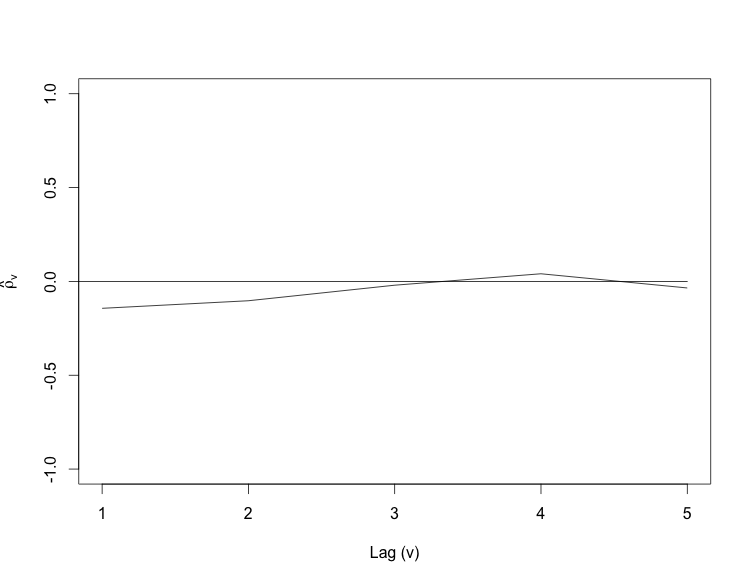
\includegraphics[scale=0.25]{./figures/PreliminariesCorrelogramGaussian} &
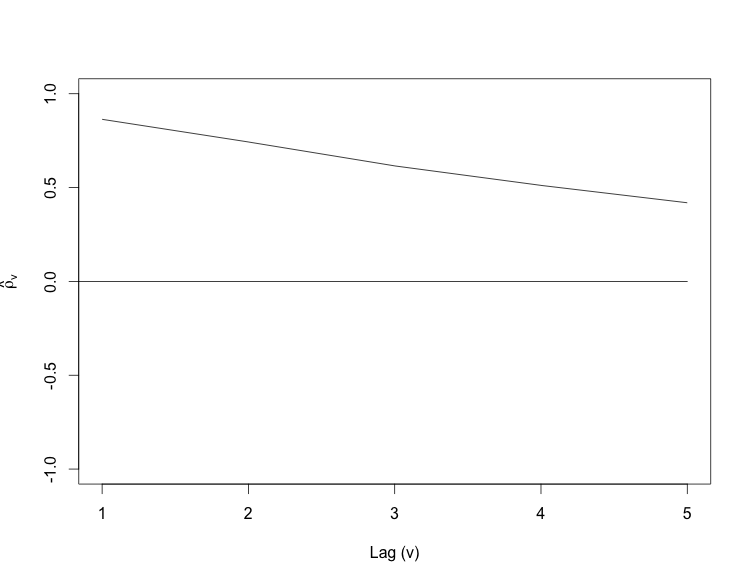
\includegraphics[scale=0.25]{./figures/PreliminariesCorrelogramTimeSerie} \\
\small (a) Correlogram for i.i.d. data & \small (b) Correlogram for a time series data \\
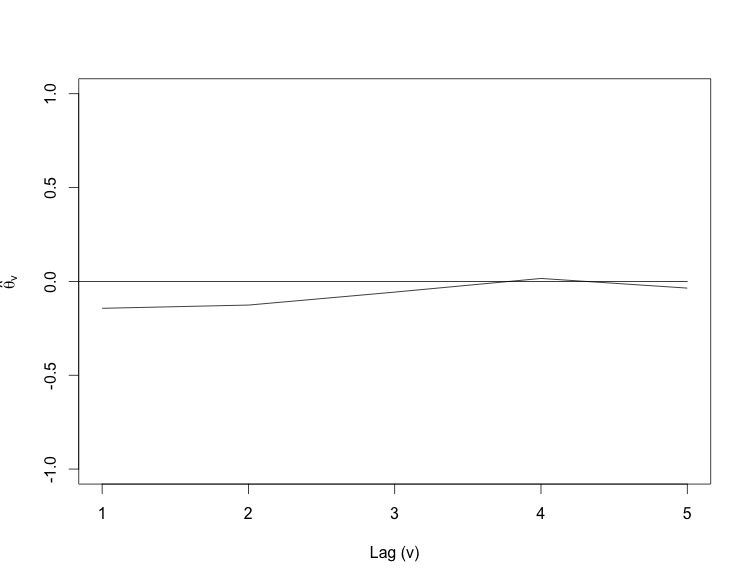
\includegraphics[scale=0.25]{./figures/PreliminariesPartialCorrelogramGaussian} &
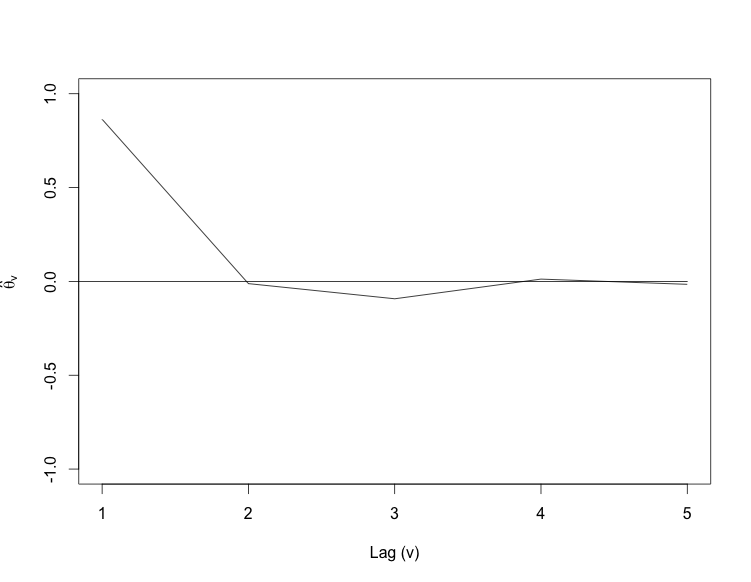
\includegraphics[scale=0.25]{./figures/PreliminariesPartialCorrelogramTimeSerie} \\
\small (c) Partial correlogram for i.i.d. data & (d) \small Partial correlogram for a time series data \\
\end{tabular}
\caption{\label{Figure:PreliminariesCorrelograms} Examples of sample correlograms and sample partial correlograms for i.i.d. and time series data. 
}
\end{center}
\end{figure}

\end{itemize}

%-----------------------------------------------------------------------------------------------
\subsubsection{Histograms and bivariate contour plots}
%-----------------------------------------------------------------------------------------------

The aim here is to use histograms and bivariate contour plots in order to get insights into the probability distributions of the proposed models. 

\begin{itemize}
\item \textbf{Histograms}: Despite the fact that this tool is quite useful in a static context, it is rather limited in dynamic models. For example, let us assume we have a time series $x_1,\ldots, x_T$ and our histogram shows that the empirical distribution of the variable when we aggregate the data samples over time looks like a mixture of Gaussian distributions. There are at least two possibilities that can give rise to this finding: 
i) $X_t$ is distributed according to a mixture of Gaussians where each Gaussian component depends on $X_{t-1}$; and ii) there is a discrete hidden variable $Z_t$ that influences $X_{t}$ and is the one responsible for generating the different mixture components. In any case, however, we could deduce that using Gaussian distributions would be appropriate.

Thus, despite its limitations in dynamic contexts, we will resort to the use of histograms whenever we find that they could shed some lights on the underlying sample distribution of the sample.

\item \textbf{Bivariate contour plots}: The contour plots of the empirical bivariate distribution of $X_t$ versus $X_{t-1}$ can show many relevant information, such as the presence of linear relationships between variables or if we can assume they are normally distributed, etc. In Figure \ref{Figure:PreliminariesBivariates}, we plot the bivariate contour plot for the i.i.d and time series data described above. As it can be seen, the bivariate contour plot for time series data shows how $X_t$ and $X_{t+1}$ seems to be distributed according to a bivariate normal with a covariance matrix that displays a strong degree of correlation. In the case of i.i.d. data, the bivariate contour plot does not reveal any temporal dependence between $X_t$ and $X_{t-1}$. 

\begin{figure} [ht!]
\begin{center}
\begin{tabular}{cc}
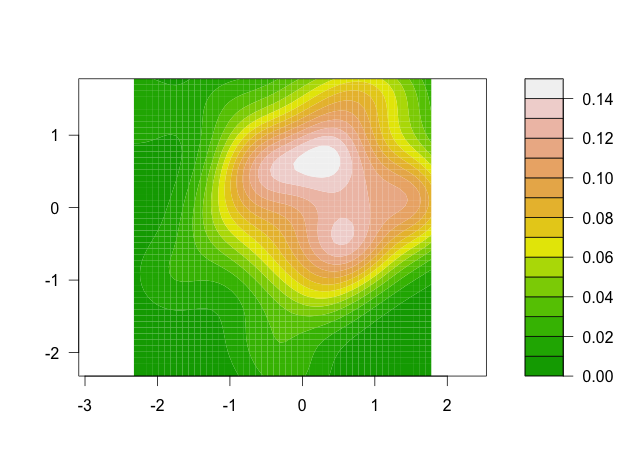
\includegraphics[scale=0.25]{./figures/PreliminariesBivariateGaussian} &
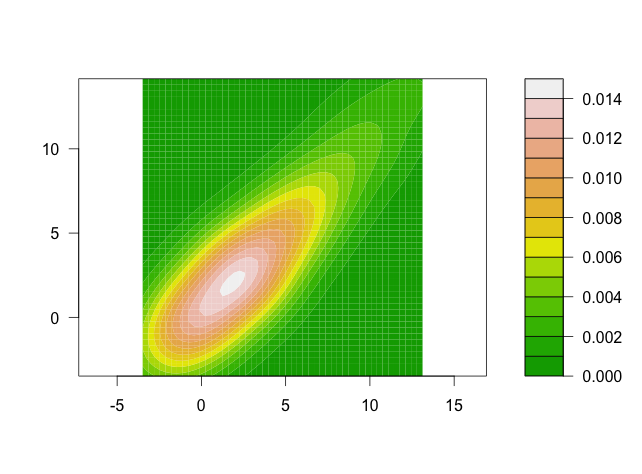
\includegraphics[scale=0.25]{./figures/PreliminariesBivariateTimeSerie} \\
(a) i.i.d. data & (b)  Time series data \\
\end{tabular}
\caption{\label{Figure:PreliminariesBivariates}Bivariate contour plots for a set of i.i.d. and time series data. 
}
\end{center}
\end{figure}

\end{itemize}

Finally, note that the usefulness of all these tools is limited due to its generative nature. That is, they do not explicitly target the prediction problem for the different use cases. After performing a proper evaluation of the considered static and dynamic models, it will be possible to re-adjust, if needed, our current assumptions. 
